

\section{Etapa 1}

\begin{figure}[H]
\centering
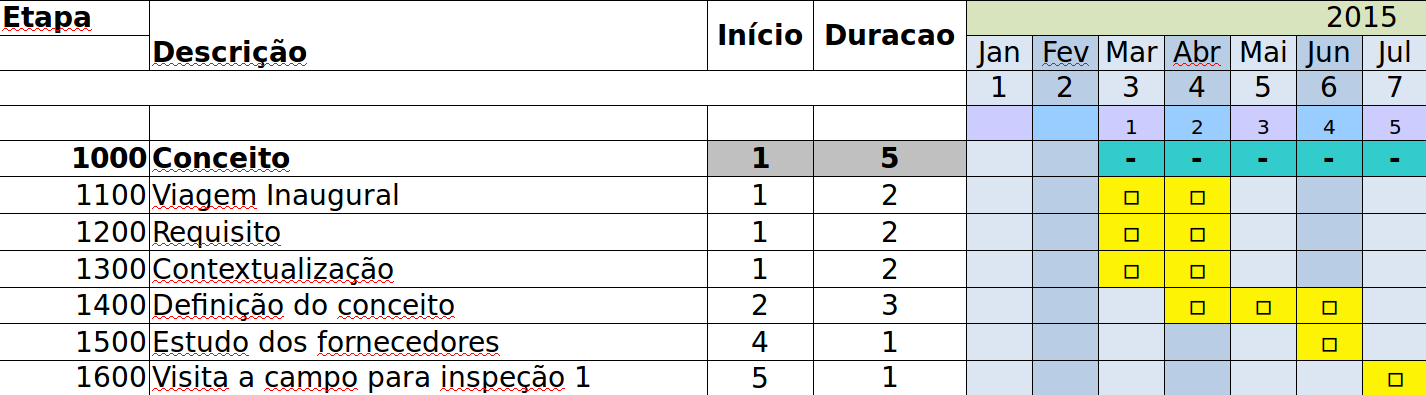
\includegraphics[width=0.9\columnwidth]{figs/etapa1}
\end{figure} 

\textbf{1000 Conceito:} A etapa 1000 do projeto foi executada como prevista. O
objetivo da etapa foi a determinação dos requisitos do problema e concepção de
possíveis soluções. Os seguintes trabalhos foram executados dentro desta etapa

\noindent
\textbf{1100 Viagem Inaugural:} Assinatura do termo inaugural do projeto e
análise em campo da problemática

Etapa executada como previsto. 

%\begin{figure}[H]
%\centering
%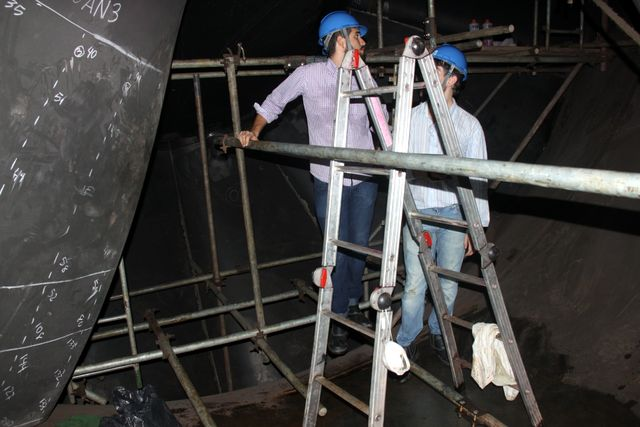
\includegraphics[width=0.6\columnwidth]{figs/img_4967}
%\caption{Pesquisadores analisando o ambiente.}
%\end{figure}

\noindent
\textbf{1200 Requisito:} Fazer levantamento dos requisitos que afetam a
instalação e utilização de um robô dentro circuito hidráulico.

Etapa executada como previsto. Foram levantados todos os requisitos de acesso,
ambiente e processo de coating.

\noindent
\textbf{1300 Contextualização:} Levantamento das tecnologias existentes no para
aplicações de revestimento em ambientes confinados.

Etapa executada como previsto. Diversas tecnologias foram pesquisadas, como o
robô scompi da hidroquebec. Nenhuma das soluções atuais atendiam os requisitos
de operação do projeto.

\noindent
\textbf{1400 Definição do conceito:} Definição de uma solução de um robô capaz
de operar no ambiente e realizar tarefas de revestimento, como ilustrado na
figura \ref{fig::conceito1}.				 .

Etapa executada como previsto. Foram levantados 3 conceitos viáveis, os quais
foram analisados chegando ao conceito proposto dentro do projeto. Utilizar um
manipu\-lador industrial, acessando o circuito hidráulico pela escotilha de
acesso, com movimenta\-ção através de trilhos modulares e alinhamento,
mapeamento e planejamento de trajetória baseado em scan 3D a laser do ambiente.

\begin{figure}
\centering
\label{fig::conceito}
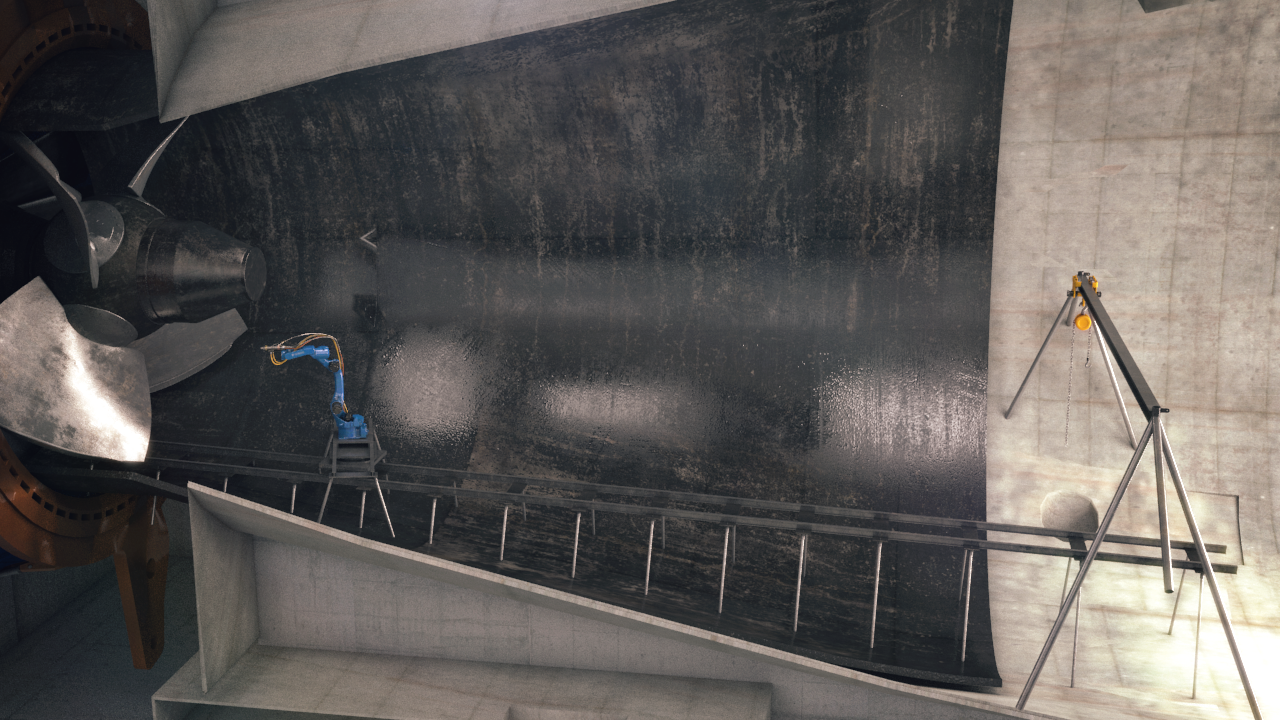
\includegraphics[width=0.9\columnwidth]{figs/turbine_evo}
\caption{Solução conceito.}
\label{fig::conceito1}
\end{figure}

\noindent
\textbf{1500 Estudo dos fornecedores:} Definição dos fornecedores do equipamento
necessário para a pesquisa

Etapa executada como previsto. Foram analisados mais de 50 modelos de
manipuladores distintos, sendo que 5 atendiam os requisitos do problema como
possíveis soluções (fig. \ref{fig::modelos_robos}).

\begin{figure}[h!]
\centering
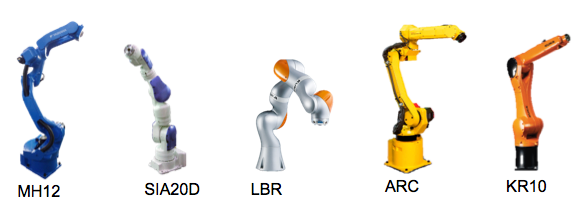
\includegraphics[width=0.9\columnwidth]{figs/robots}
\caption{Possíveis modelos de manipuladores que atendem os requisitos.}
\label{fig::modelos_robos}
\end{figure}

\noindent
\textbf{1600 Visita a campo para inspeção 1:} foi realizada uma visita inicial
a campo para juntamente com revisão bibliográfica sobre o tema “desgaste”
coletar dados de campo através de inspeção nas pás das turbinas. Essas inspeções
foram realizadas ao longo do projeto para confrontar com o que existe na
bibliografia.


\section{Etapa 02}

\begin{figure}[H]
\centering
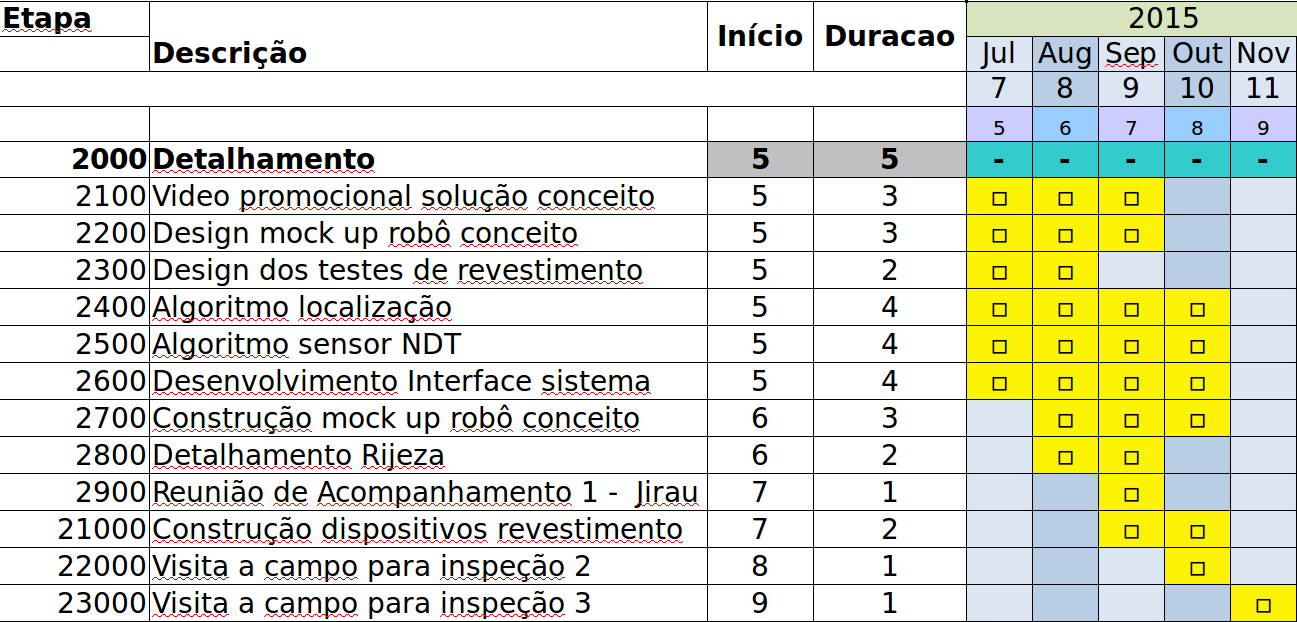
\includegraphics[width=0.9\columnwidth]{figs/etapa2}
\end{figure} 

\noindent
\textbf{2000 Detalhamento:} A etapa 2000 do projeto foi executada existindo
variações entre previsto e executado. O objetivo da etapa foi a análise das
proposições mediante estudos teóricos e design detalhado da possível solução e sistema

\noindent
\textbf{2100 Video promocional solução conceito:} Animação 3D da solução
conceito

Houve atraso no processo de contratação e aprovação do script. A tarefa foi
executada com 3 meses de atraso. Entretanto, o mesmo não impactou no projeto,
pois não era uma tarefa de pré-requisito.

\noindent
\textbf{2200 Design mock up robô conceito:} Design em CAD / Solidworks do
conceito do robô

Tarefa executada como prevista. Foram realizado diversos designs para possíveis
bases para a solução conceito, assim como análises geométricas, cinemática,
dinâmica e de manipulabilidade para definir o manipulador, como ilustrado na
figura \ref{fig::ex_cad}.

\begin{figure}
\centering
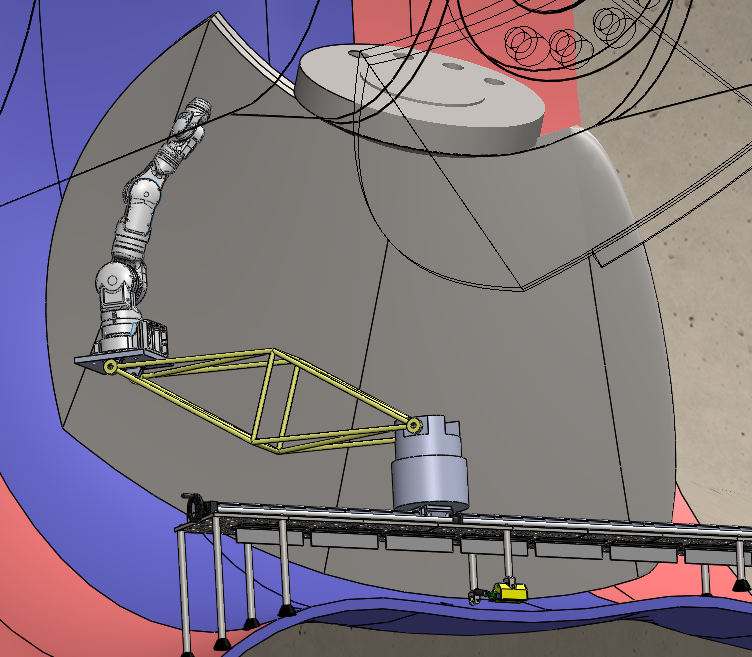
\includegraphics[width=0.6\columnwidth]{figs/EMMA_Base_Conceito_PRR}
\caption{Possível base para o manipulador dentro do ambiente do circuito
hidráulico.}
\label{fig::ex_cad}
\end{figure} 


\noindent
\textbf{2300 Design dos testes de revestimento:} Foram definidos os testes e a
sequência de testes a serem realizados para cada modificação de equipamento e
cada material de coating utilizado.

\noindent
\textbf{2400 Algoritmo de localização:} definir o algoritmo/técnica que irá
localizar o robô com relação a turbina.

Tarefa executada como prevista. Foi determinado que o melhor e mais preciso
método é escanear o robô e a pá com um laser de metrologia e a estimar posição
relativa das nuvens de pontos resultante, ilustrada na figura
\ref{fig::pos_rel}.

\begin{figure}[H]
\centering
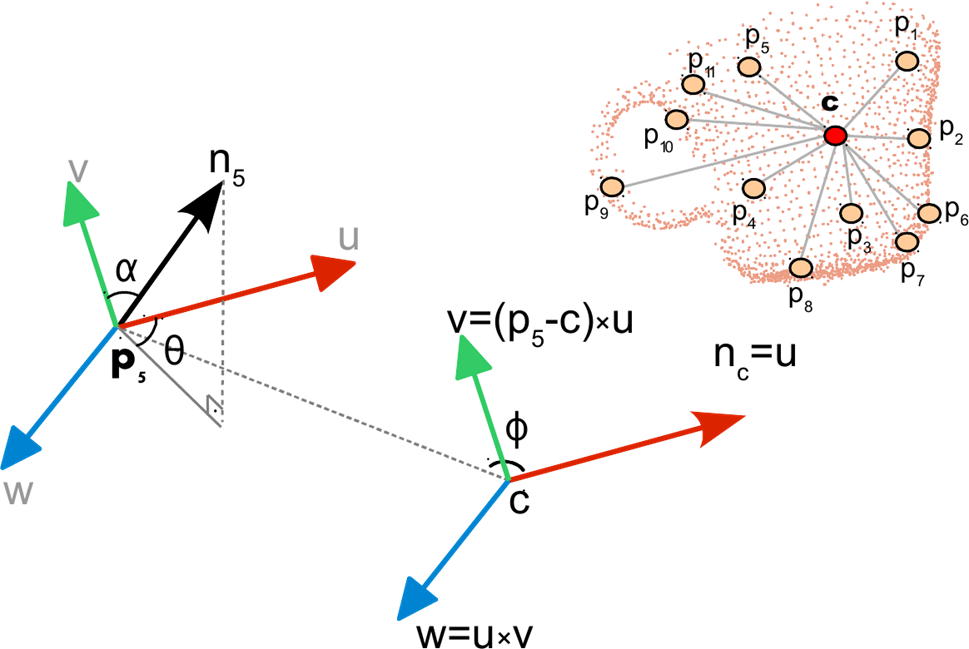
\includegraphics[width=0.6\columnwidth]{figs/pc_position}
\caption{Posição relativa entre duas nuvens de pontos.}
\label{fig::pos_rel}
\end{figure} 

\noindent
\textbf{2500 Algoritmo sensor NDT:} Algoritmo que irá avaliar e mapear a
qualidade do revestimento.

Tarefa executada como prevista. Foi determinado que o método mais eficiente é
utilizar um humano para rapidamente realizar uma amostragem de alguns pontos com
sensor ultra-som manual. A solução robótica seria em uma alusão “matar um mosquito com basuca”.

\noindent
\textbf{2600 Desenvolvimento Interface sistema:} Interface gráfica de controle e
utilização do sistema

Essa tarefa foi estendida para 8 meses, se tornando uma tese de mestrado dada
sua complexidade. A solução conceito possui um volume muito grande de interação
e informação para o usuário. Logo, adotou-se um estudo metódico,
estabelecendo-se toda a metodologia para determinar a interface e como cada
informação será representada.

\noindent
\textbf{2700 Construção mock up robô conceito:} Construção do mock up do robô
que aplica o revestimento

Tarefa executada como previsto. Foi construído todo o ambiente do circuito
hidráulico e manipulador através de impressão 3D em uma escala 1:20, ilustrado
pela figura \ref{fig::maquete}.

\begin{figure}[h!]
\centering
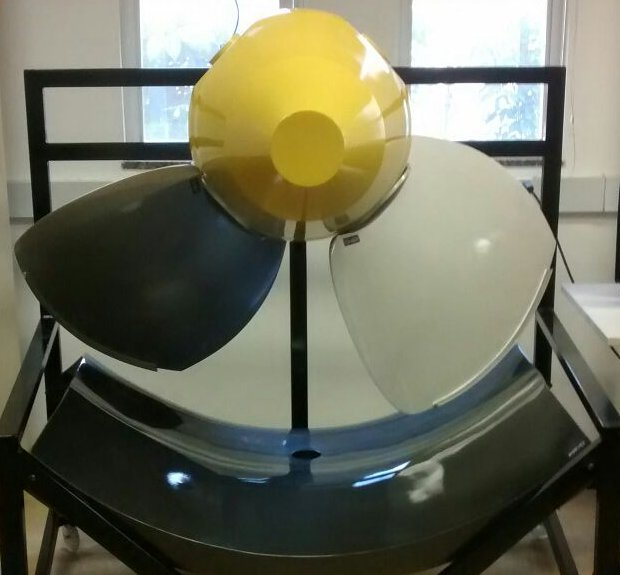
\includegraphics[width=0.6\columnwidth]{figs/maquete}
\caption{Maquete utilizada no desenvolvimento do conceito.}
\label{fig::maquete}
\end{figure} 

  
\noindent
\textbf{2800 Detalhamento RIJEZA:} Foram realizados projetos e detalhamento de
dispositivos necessários para realização dos testes definidos na etapa de
design dos testes baseando-se nas modificações necessárias para adequação do
equipamento de jateamento e coating no ambiente definido e no uso dos materiais
selecionados para revestimento.

\noindent
\textbf{2900 Reunião de acompanhamento:} Durante a reunião foram expostas as
soluções de sistemas robóticas do estado da arte para realização de tarefas
similares às que serão realizadas durante a implantação	do projeto EMMA. Foram,
também, esclarecidas questões técnicas com as equipes da ESBR e RIJEZA (fig.
\ref{fig::reuniao}).

\noindent
\textbf{21000 Construção dispositivos revestimento:} Etapa de dedicada para a
fabricação de peças e montagem dos dispositivos projetados na etapa de
detalhamento dos dispositivos (etapa 2300).


\noindent
\textbf{22000 Visita a campo para inspeção 2:} Visita realizada na UHE Jirau
para verificação de acessos ao circuito hidráulico realizada com a fim de
complementar o estudo de definição das modificações que seriam necessárias para
serem realizadas nos equipamentos e prever movimentos e alocações dos
equipamentos dentro do circuito.


\noindent
\textbf{23000 Visita a campo para inspeção 3:} Visita realizada na UHE Jirau,
nas máquinas 29 e 39, com a finalidade de inspecionar o desgaste das pás,
complementando o estudo de definições de testes necessários para qualificação
dos revestimentos.

\begin{figure}[h!]
\centering
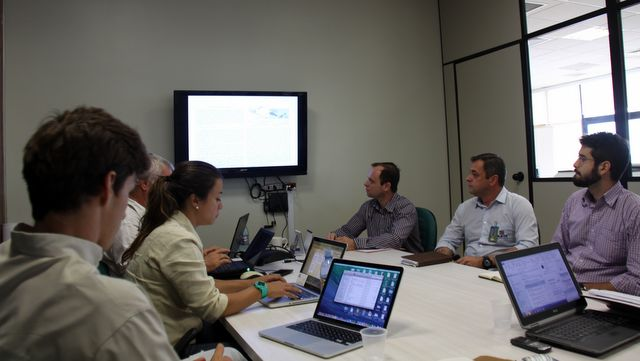
\includegraphics[width=0.6\columnwidth]{figs/img_4836}
\caption{Reunião de acompanhamento em Jirau.}
\label{fig::reuniao}
\end{figure} 

\section{Etapa 03} 

\begin{figure}[H]
\centering
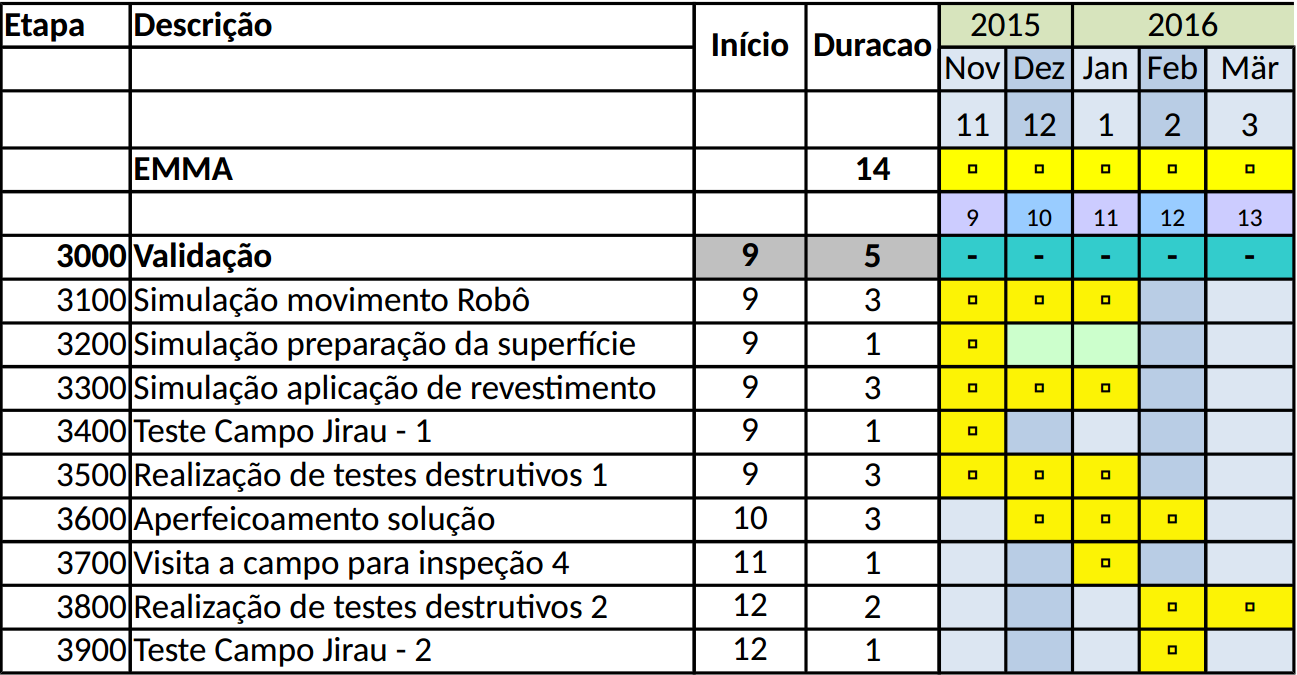
\includegraphics[width=0.9\columnwidth]{figs/etapa03_final_gisele}
\end{figure} 

\noindent
\textbf{3000 Validação:} A etapa 3000 do projeto foi executada existindo
variações entre previsto e executado. O objetivo da etapa é a validação da
solução detalhada através de simulação e experimentos.

\noindent
\textbf{3100 Simulação movimento robô:} 
Simulação dos movimentos do robô sobre a turbina, verificando limites e singularidades

Tarefa executada como prevista. Foi utilizado o simulador OpenRAVE, que provê
um ambiente de simulação para testes, desenvolvimento e implementação de
algoritmos de planejamento de movimento em aplicações de robótica
\noindent
\textbf{3200 Simulação preparação de superfície:}
Testes para avaliar a modificação do procedimento de jateamento para a sua adequação ao ambiente proposto no projeto;

\noindent
\textbf{3300 Simulação aplicação revestimento:}

Aplicação em amostras de testes para qualificação de materiais e procedimento de aspersão para posterior avaliação comparativa do desempenho dos sistemas de revestimentos.


\noindent
\textbf{3400 Teste de Campo Jirau 01:} Teste da solução  em Jirau sobre
condições reais de operação.

Tarefa executada antes do previsto. Os testes de campo foram executados durante
a viagem de acompanhamento que ocorreu na etapa 2900. Foram testados os
conceitos de acoplamento magnético (fig \ref{fig::teste_base}) e mapeamento 3D
com laser scanner.
\begin{figure}
\centering
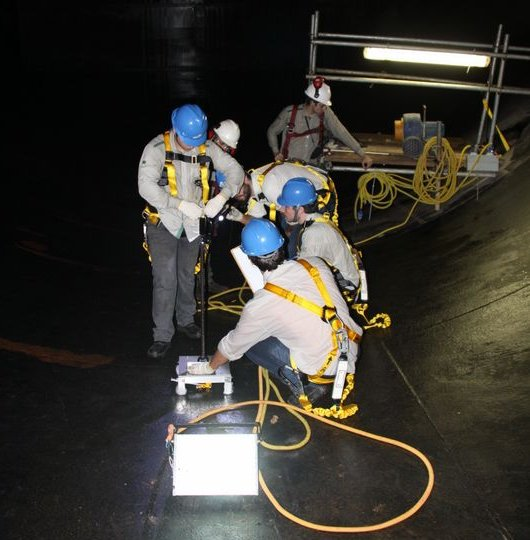
\includegraphics[width=0.6\columnwidth]{figs/base}
\caption{Teste de campo com a base  magnética}
\label{fig::teste_base}
\end{figure}

\noindent
\textbf{3500 Realização dos testes destrutivos – 1}
Realização dos testes para verificar se o revestimento mantém as 
características técnicas exigidas para a aplicação após mudanças de parâmetros. Nessa etapa foram realizados os testes de qualificação dos revestimentos antes e após mudanças de parâmetros e realização de ensaios destrutivos comparativos normatizados. 

\noindent
\textbf{3600 Aperfeiçoamento da solução:}
Aperfeiçoamento da solução baseado nos resultados dos testes de campo. 

Tarefa atrasada em 1 mês com impacto de atraso de 1 mês no projeto. O cálculo da
posição relativa entre o robô e a pá, baseado em dados reais do sensor de
metrologia testado em campo, está com um erro de 0,1-0,2 graus o que resulta em
um erro de posição da extremidade do manipulador na ordem de centímetros. A
ordem de grandeza desejada para poder fazer reparo do perfil hidráulico é em
milímetros. Logo, as técnicas de alinhamento continuando sendo aprimoradas.

% \begin{figure}
% \centering
% 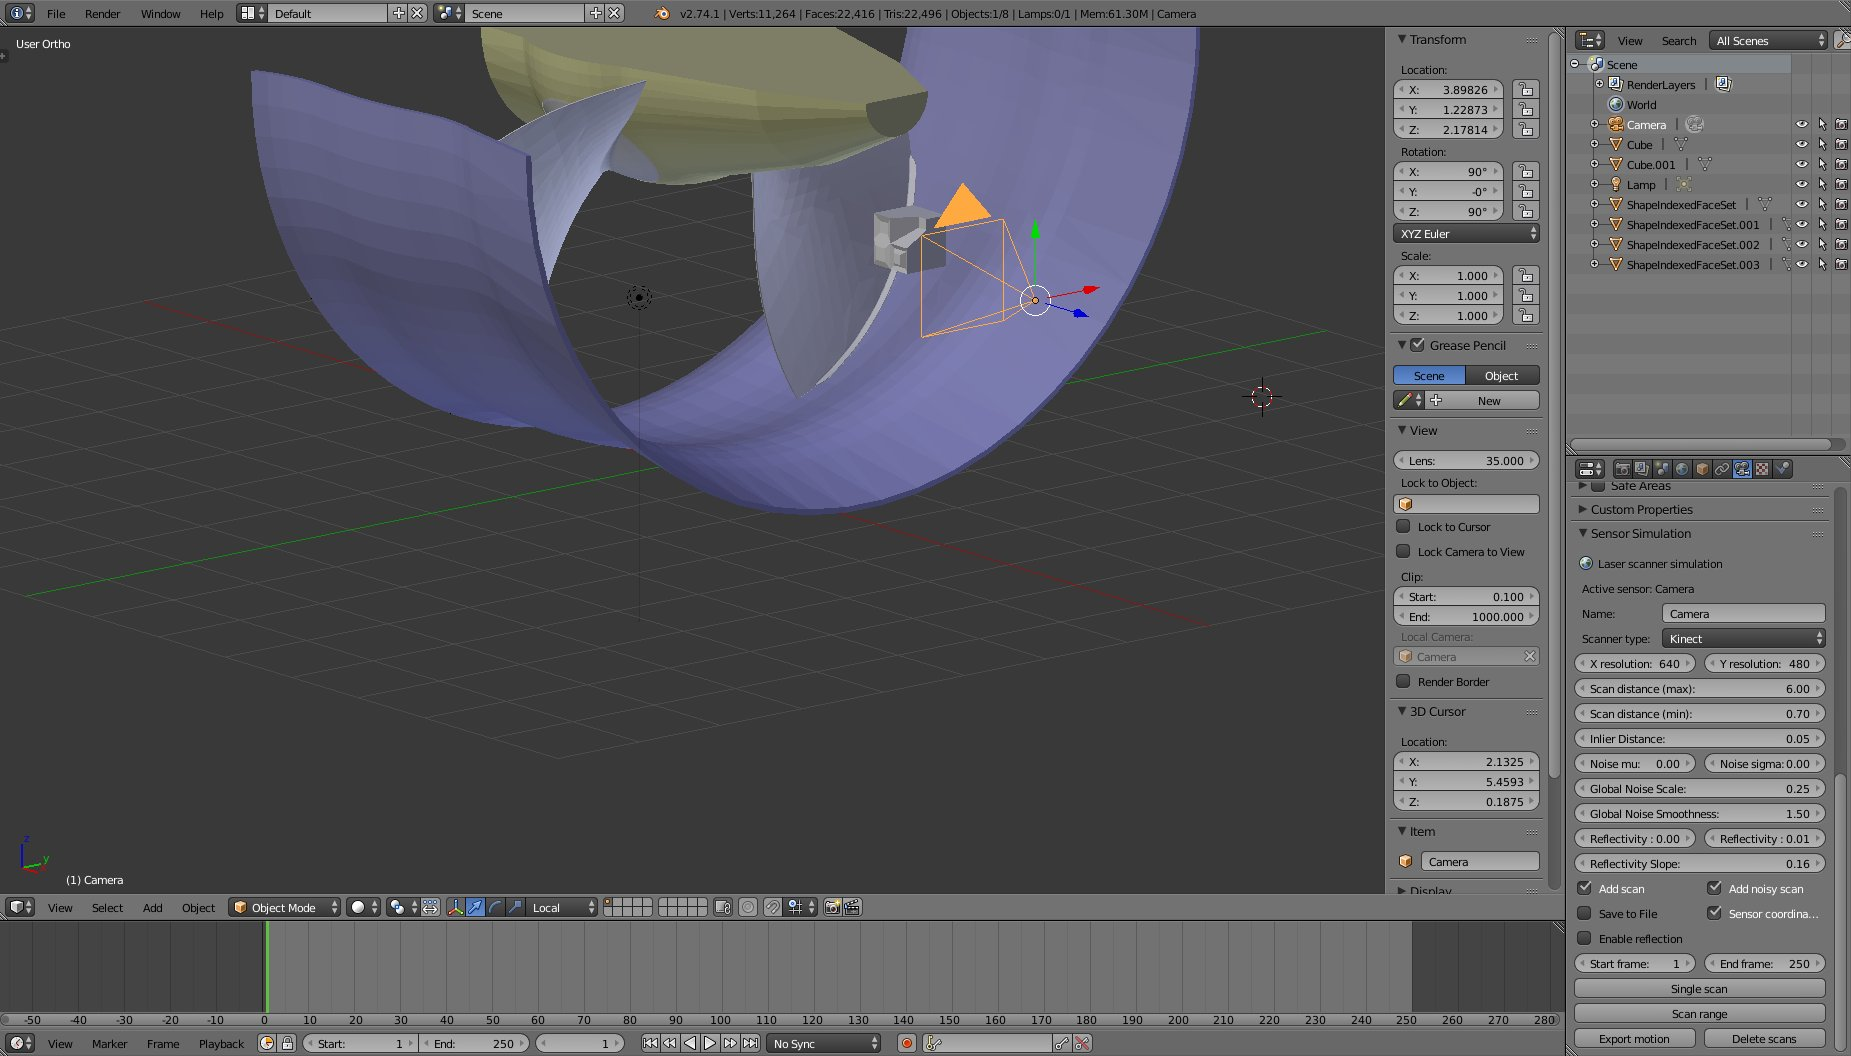
\includegraphics[width=0.6\columnwidth]{figs/blensor_screen}
% \caption{Estimando posição relativa usando um simulador para análise dos
% resultados.}
% \end{figure} 



\noindent
\textbf{3700 – Visita a campo para Inspeção 4}

A inspeção nas pás é realizada com o fim de avaliar o progresso do desgate nas superfícies das
pás e também determinar o tipo e a severidade em cada região da pá.

\noindent
\textbf{3800  Visita a campo para Inspeção 4:}
A inspeção nas pás é realizada com o fim de avaliar o progresso do desgate nas superfícies das pás e também determinar o tipo e a severidade em cada região da pá. 

\noindent
\textbf{3900 Realização dos testes destrutivos 2:}

Continuação da realização dos testes destrutivos após anális dos resultados prévio. As amostras que estvam em atraso na antrega dos resultados de cavitação foram realizadas nessa etapa. Também foram testes de aplicação de revestimento orgânico para melhoria das características do revestimento.


\noindent
\textbf{3900 Teste de Campo Jirau 02:} Teste da solução  em Jirau sobre
condições reais de operação.

Tarefa cancelada. As informações necessárias para esta fase do
projeto foram coletadas durante o teste de campo 01. 

\section{Etapa 04} 

\begin{figure}[H]
\centering
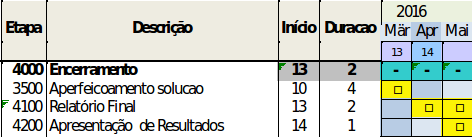
\includegraphics[width=0.9\columnwidth]{figs/etapa4}
\end{figure} 

\noindent
\textbf{4000 Encerramento:} A etapa 4000 do projeto foi executada existindo
variações entre previsto e executado. Inicialmente esta etapa era para ser
iniciada em março e encerrada em abril. Entretanto a mesma sofreu um atraso de 1
mês devido a necessidade de mais tempo para encerrar a etapa de aperfeiçoamento
da solução. O objetivo da etapa é preparar os relatórios finais e artigos acadêmicos do projeto.

\noindent
\textbf{4100 Relatório Final:} Relatório de encerramento do projeto no formato
P\&D ANEEL e artigos acadêmicos.

Etapa executada como prevista. 

\noindent
\textbf{4200 Apresentação dos resultados:} Difusão dos conhecimentos.

Etapa executada como prevista. A difusão do conhecimento se deu por meio de dois
artigos acadêmicos e apresentação dos resultados na UHE Jirau.
